\documentclass[10pt,a4paper]{report}
\usepackage[utf8]{inputenc}
\usepackage[T1]{fontenc}
\usepackage[ngerman]{babel}
\usepackage{amsmath}
\usepackage{amsfonts}
\usepackage{amssymb}
\usepackage{makeidx}
\usepackage{graphicx}
\usepackage{fancyhdr}
\usepackage{color}
\usepackage{listings}
\usepackage{hyperref}
\usepackage{svg}
\title{Dokumentation RGB-Sensor}
\author
\pagestyle{fancy}

\graphicspath{ {./bilder/} }

\lstloadlanguages{bash, Python}
\lstset{alsolanguage=bash}
\lstset{alsolanguage=Python}

\lhead{\slshape \rightmark}
\chead{}
\rhead{\slshape \leftmark}

\lfoot{}
\cfoot{\thepage}
\rfoot{}

\renewcommand{\headrulewidth}{0.4pt}
\renewcommand{\footrulewidth}{0pt}

\lstset{language=Python,
	basicstyle=\scriptsize\ttfamily,
	keywordstyle=\color{red}\bfseries,
	identifierstyle=\color{blue},
	commentstyle=\color{DarkGreen},
	stringstyle=\ttfamily,
	breaklines=true,
	numbers=left,
	numberstyle=\tiny,
	frame=single,
	backgroundcolor=\color{myGrey},
	caption={Python-Code},
	tabsize=2}
\definecolor{myGrey}{gray}{0.9}
\definecolor{DarkGreen}{rgb}{0.2,0.5,0.6}





\begin{document}
	\maketitle
	\newpage
	\tableofcontents
	\newpage
	
	\chapter{Farberkennung}
	\newpage
	\section{Aufsetzen und Auslesung}
	\subsection{Raspberry Pi aufsetzen:}
	Um den Raspberry Pi aufzusetzen, muss man diesen zuerst über ein HDMI-Kabel oder über SSH verbinden, sich 			einloggen (Benutzername: pi, Passwort:ilovecolors) und 
	mit einem Netzwerk verbinden, wo der Laptop/Computer auch angeschlossen ist. Daraufhin kann man die Ausführung 		starten, indem man in der Console des Raspberry Pi's \\ "python main.py *hier die lokale IP-Adresse eingeben*" 		\\ schreibt und auf 'Enter' drückt.
	\begin{figure}[h]
	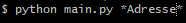
\includegraphics{beispiel.png}
	\end{figure}
	\\
	Jetzt sollte der Raspberry Pi aufgesetzt sein.
	\\
	\subsection{Client-Seite (Computer oder Laptop)}
	Wenn der PC im gleichen Netzwerk ist und sie den ersten Schritt vollendet haben, können sie die Python-Datei 		'client.py' ausführen und dort die lokale IP-Adresse des Pi's eingeben und sich verbinden.

	\begin{figure}[h]
	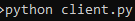
\includegraphics{beispiel2.png}
	\end{figure}	
	!!!Achtung, es ist wichtig, dass sie Python 3 auf ihrem PATH installiert haben und in dem Projektordner sind, 
	damit die Datei ausgeführt werden kann!!! 
	\\
	Mit dem Knopf 'Verbinden zum Server' verbinden sie sich mit dem Raspberry Pi. Der Knopf 'Farberkennung' 
	schickt eine Anfrage an den Raspberry Pi, der dann die Farbe erkennt und diese dann zurückschickt. Die erkannte 
	Farbe sieht man dann in der Liste.
	
	\newpage
	
	\chapter{Quellcode}
	
	
	\newpage
	\section{Main.py}
	\begin{lstlisting}
		import cv2 as cv
		import socket
		import sys
		
		from null_preview import *
		from picamera2 import *
		
		#Setup des Sockets und der Kamera
		currentColor = ""
		lastColor = ""
		sock = socket.socket(socket.AF_INET, socket.SOCK_STREAM)
		server_address = (str(sys.argv[1]), 18769)
		print('starting up on {} port {}'.format(*server_address))
		sock.bind(server_address)
		picam2 = Picamera2()
		preview = NullPreview(picam2)
		picam2.configure(picam2.preview_configuration(main={"size":(640, 480)}))
		picam2.start()
		sock.listen(1000)
		connection, client_address = sock.accept()
		
		
		#Bild der Kamera wird als Numpy Array ausgelesen
		def evaluate_current_frame():
		img = picam2.capture_array()
		
		img = cv.cvtColor(img, cv.COLOR_BGR2RGB)
		
		Z = img.reshape((-1,3))
		# Konventiert zu np.float32
		Z = np.float32(Z)
		# Definiton der Kriterien der Farbdominanz, Anzahl an dominanten Farben(K) und anschliessend wird der KMeans Algorithmus angewendet
		criteria = (cv.TERM_CRITERIA_EPS + cv.TERM_CRITERIA_MAX_ITER, 10, 1.0)
		K = 1
		ret,label,center=cv.kmeans(Z,K,None,criteria,10,cv.KMEANS_RANDOM_CENTERS)
		# Zurueck zu unsigned int, damit das Buffer mit dem Bild wieder zu der urspruenglichen Form zurueckkehrt
		center = np.uint8(center)
		res = center[label.flatten()]
		res2 = res.reshape((img.shape))
		
		
		#Trennt Farbkanaele
		(b, g, r) = cv.split(res2)
		
		b_mean = np.mean(b)
		g_mean = np.mean(g)
		r_mean = np.mean(r)
		
		# Bestimmt die prominenteste Farbe und setzt die Variable
		if (b_mean > g_mean and b_mean > r_mean):
		currentColor = "blue"
		elif (g_mean > r_mean and g_mean > b_mean):
		currentColor = "green"
		else:
		currentColor = "red"
		
		#Sendet String an den Client zurueck		
		
		message = currentColor.encode()
		connection.sendall(message)
		
		def close_socket():
		sock.close()
		
		while True:
		try:
		data = connection.recv(16)
		dataBuffer = data.decode('utf-8')
		if(dataBuffer == "getcolor"):
		evaluate_current_frame()
		elif(dataBuffer == "closesocket"):
		close_socket()
		
		
		except OSError:
		print("STOPPED")
		sock.close()
		break
		
		except KeyboardInterrupt:
		print("STOPPED")
		sock.close()
		break
	\end{lstlisting}
	\newpage
	
	\section{client.py}
	\begin{lstlisting}
import socket
import sys
import tkinter as tk

ip_was_false = True

i = 1
#Socket definieren
sock = socket.socket(socket.AF_INET, socket.SOCK_STREAM)

getColorFuncName = "getcolor"
sockCloseFuncName = "closesocket"

#Funktion zum Verbinden mit dem Raspberry Pi
def connect_to_server():
    try:
        print(ip_var.get())
        server_address = (ip_var.get(), 18769)
        print('connecting to {} port {}'.format(*server_address))
        sock.connect(server_address)
    except Exception:
        global ip_was_false
        if (ip_was_false == True):
            label2 = tk.Label(root, text = "Falsche IP-Adresse!", fg = '#ff0000')
            label2.pack()
            ip_was_false = False

#Abfrage der derzeitigen Farbe
def request_color():
    message = getColorFuncName.encode()
    sock.sendall(message)

    data = sock.recv(16)
    global i
    lb1.insert(i, data.decode('utf-8'))
    i = i + 1

#Schliessen des Sockets nach Schliessen des Programms
def close_socket():
    message = sockCloseFuncName.encode()
    sock.sendall(message)

#Definition des Fensters und des Inhalts
root = tk.Tk()
root.geometry("250x170")

ip_var = tk.StringVar()

label1 = tk.Label(root, text="RGB-Sensor-System")
label1.pack()

ip_feld = tk.Entry(root, textvariable = ip_var)
ip_feld.pack()

schaltf1 = tk.Button(root, text="Verbinde zum Server", command=connect_to_server)
schaltf1.pack()

schaltf2 = tk.Button(root, text="Farberkennung", command=request_color)
schaltf2.pack()

lb1 = tk.Listbox()

root.mainloop()

		
	\end{lstlisting}
\end{document}